%\documentclass{beamer}
\documentclass[handout]{beamer}

% packages
\usepackage[T1]{fontenc}
\usepackage{lmodern}
\usepackage{amsmath}
\usepackage{amssymb}
\usepackage{graphicx}
\usepackage[justification=centering]{caption}
\usepackage{fontawesome5}
\usepackage{color}
\usepackage{minted}
\usepackage{xcolor}
\usepackage{hyperref}
\usepackage{geometry}
\usepackage{changepage}
\usepackage{booktabs}
\usepackage[framemethod=tikz]{mdframed}

\definecolor{codebg}{RGB}{240, 242, 244}
\mdfdefinestyle{code}{
  backgroundcolor=codebg,
  roundcorner=5pt,
  innerleftmargin=0,
  innerrightmargin=0,
  linewidth=0
}
\surroundwithmdframed[style=code]{minted}

\graphicspath{{images/}}

\newcommand{\tabitem}{~~\llap{\textbullet}~~}

\usetheme{zds}

% details ----------------------------------------------------------------------

\title{Deep Dive into Pin Control\\in Zephyr}
\author{
  \texorpdfstring{
    Gerard Marull-Paretas\\
    \href{mailto:gerard.marull@nordicsemi.no}{gerard.marull@nordicsemi.no}
  }{Gerard Marull-Paretas}
}
\institute{Nordic Semiconductor ASA}
\date{9\textsuperscript{th} June 2022}

% document ---------------------------------------------------------------------

\begin{document}

% section: title & toc ---------------------------------------------------------

\begin{frame}[plain]
  \titlepage{}
\end{frame}

\begin{frame}
  \frametitle{Outline}
  \tableofcontents
\end{frame}

% section: introduction --------------------------------------------------------

\section{Introduction}

\begin{frame}
  \begin{center}
    \Huge \textbf{Introduction}
  \end{center}
\end{frame}

\begin{frame}
  \frametitle{What is pin control?}

  \begin{itemize}
    \item<1-> Pin control refers to the hardware blocks that control
          \textbf{pin multiplexing} and \textbf{pin configuration parameters},
          e.g.\ pull-up/down, drive mode, slew-rate, etc.
    \item<2-> \textbf{Essential} for \textbf{SoC peripherals} that have a
          physical interface, e.g.\ I2C, SPI, UART, etc.
    \item<3-> The way pin control is implemented in hardware is
          \textbf{vendor/SoC specific}, i.e.\ non-portable
  \end{itemize}

  \begin{figure}
    \centering
    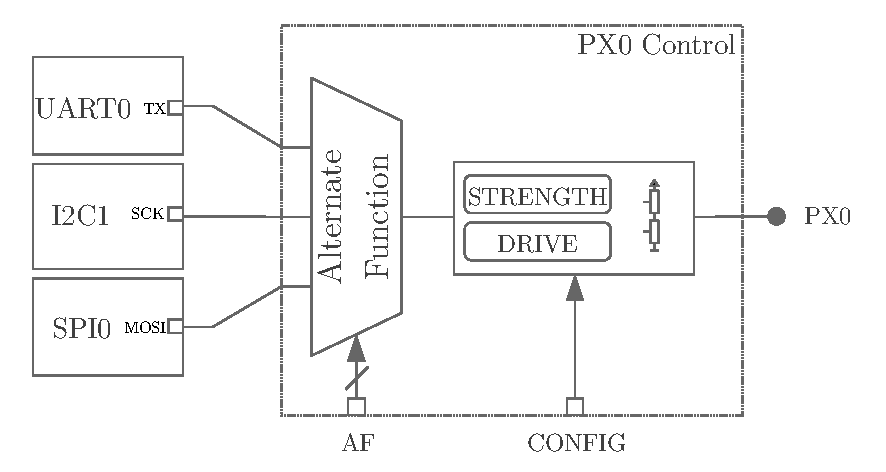
\includegraphics[scale=0.4]{hw-cent-control}
    \caption{Example of pin control centralized into a single per-pin block}
  \end{figure}
\end{frame}

\begin{frame}
  \frametitle{Pin control vs. GPIO}

  \begin{itemize}
    \item<1-> Some functionality covered by a pin controller driver
          \textbf{overlaps} with GPIO drivers, e.g.\ setting pull-up resistor
    \item<2-> The main purpose of \textbf{pin control} is to perform both
          \textbf{signal multiplexing} and \textbf{pin configuration}
          (e.g.\ slew-rate) required for the correct operation of a
          \textbf{peripheral}
    \item<3-> \textbf{GPIO} drivers are for \textbf{general purpose control} of
          a pin, that is, when its logic level is read or
          \textbf{controlled manually}
    \item<4-> \textbf{GPIO} can be usually seen as a
          \textbf{subset of pin control}. In the future GPIO drivers could
          \textbf{re-use} pin control infrastructure
  \end{itemize}
\end{frame}

\begin{frame}
  \frametitle{Pin Control in Zephyr < 3.1}

  \begin{itemize}
    \item<1-> Each \textbf{vendor} implemented its \textbf{own} solution
    \item<2-> \textbf{\texttt{pinmux}} API existed, but had
          \textbf{design limitations} and was \textbf{not always used}
    \item<3-> \textbf{Custom} Devicetree representations, some platforms did not
          even use Devicetree but harcoded
          \textbf{configuration in board C code}
  \end{itemize}

  \begin{figure}
    \centering
    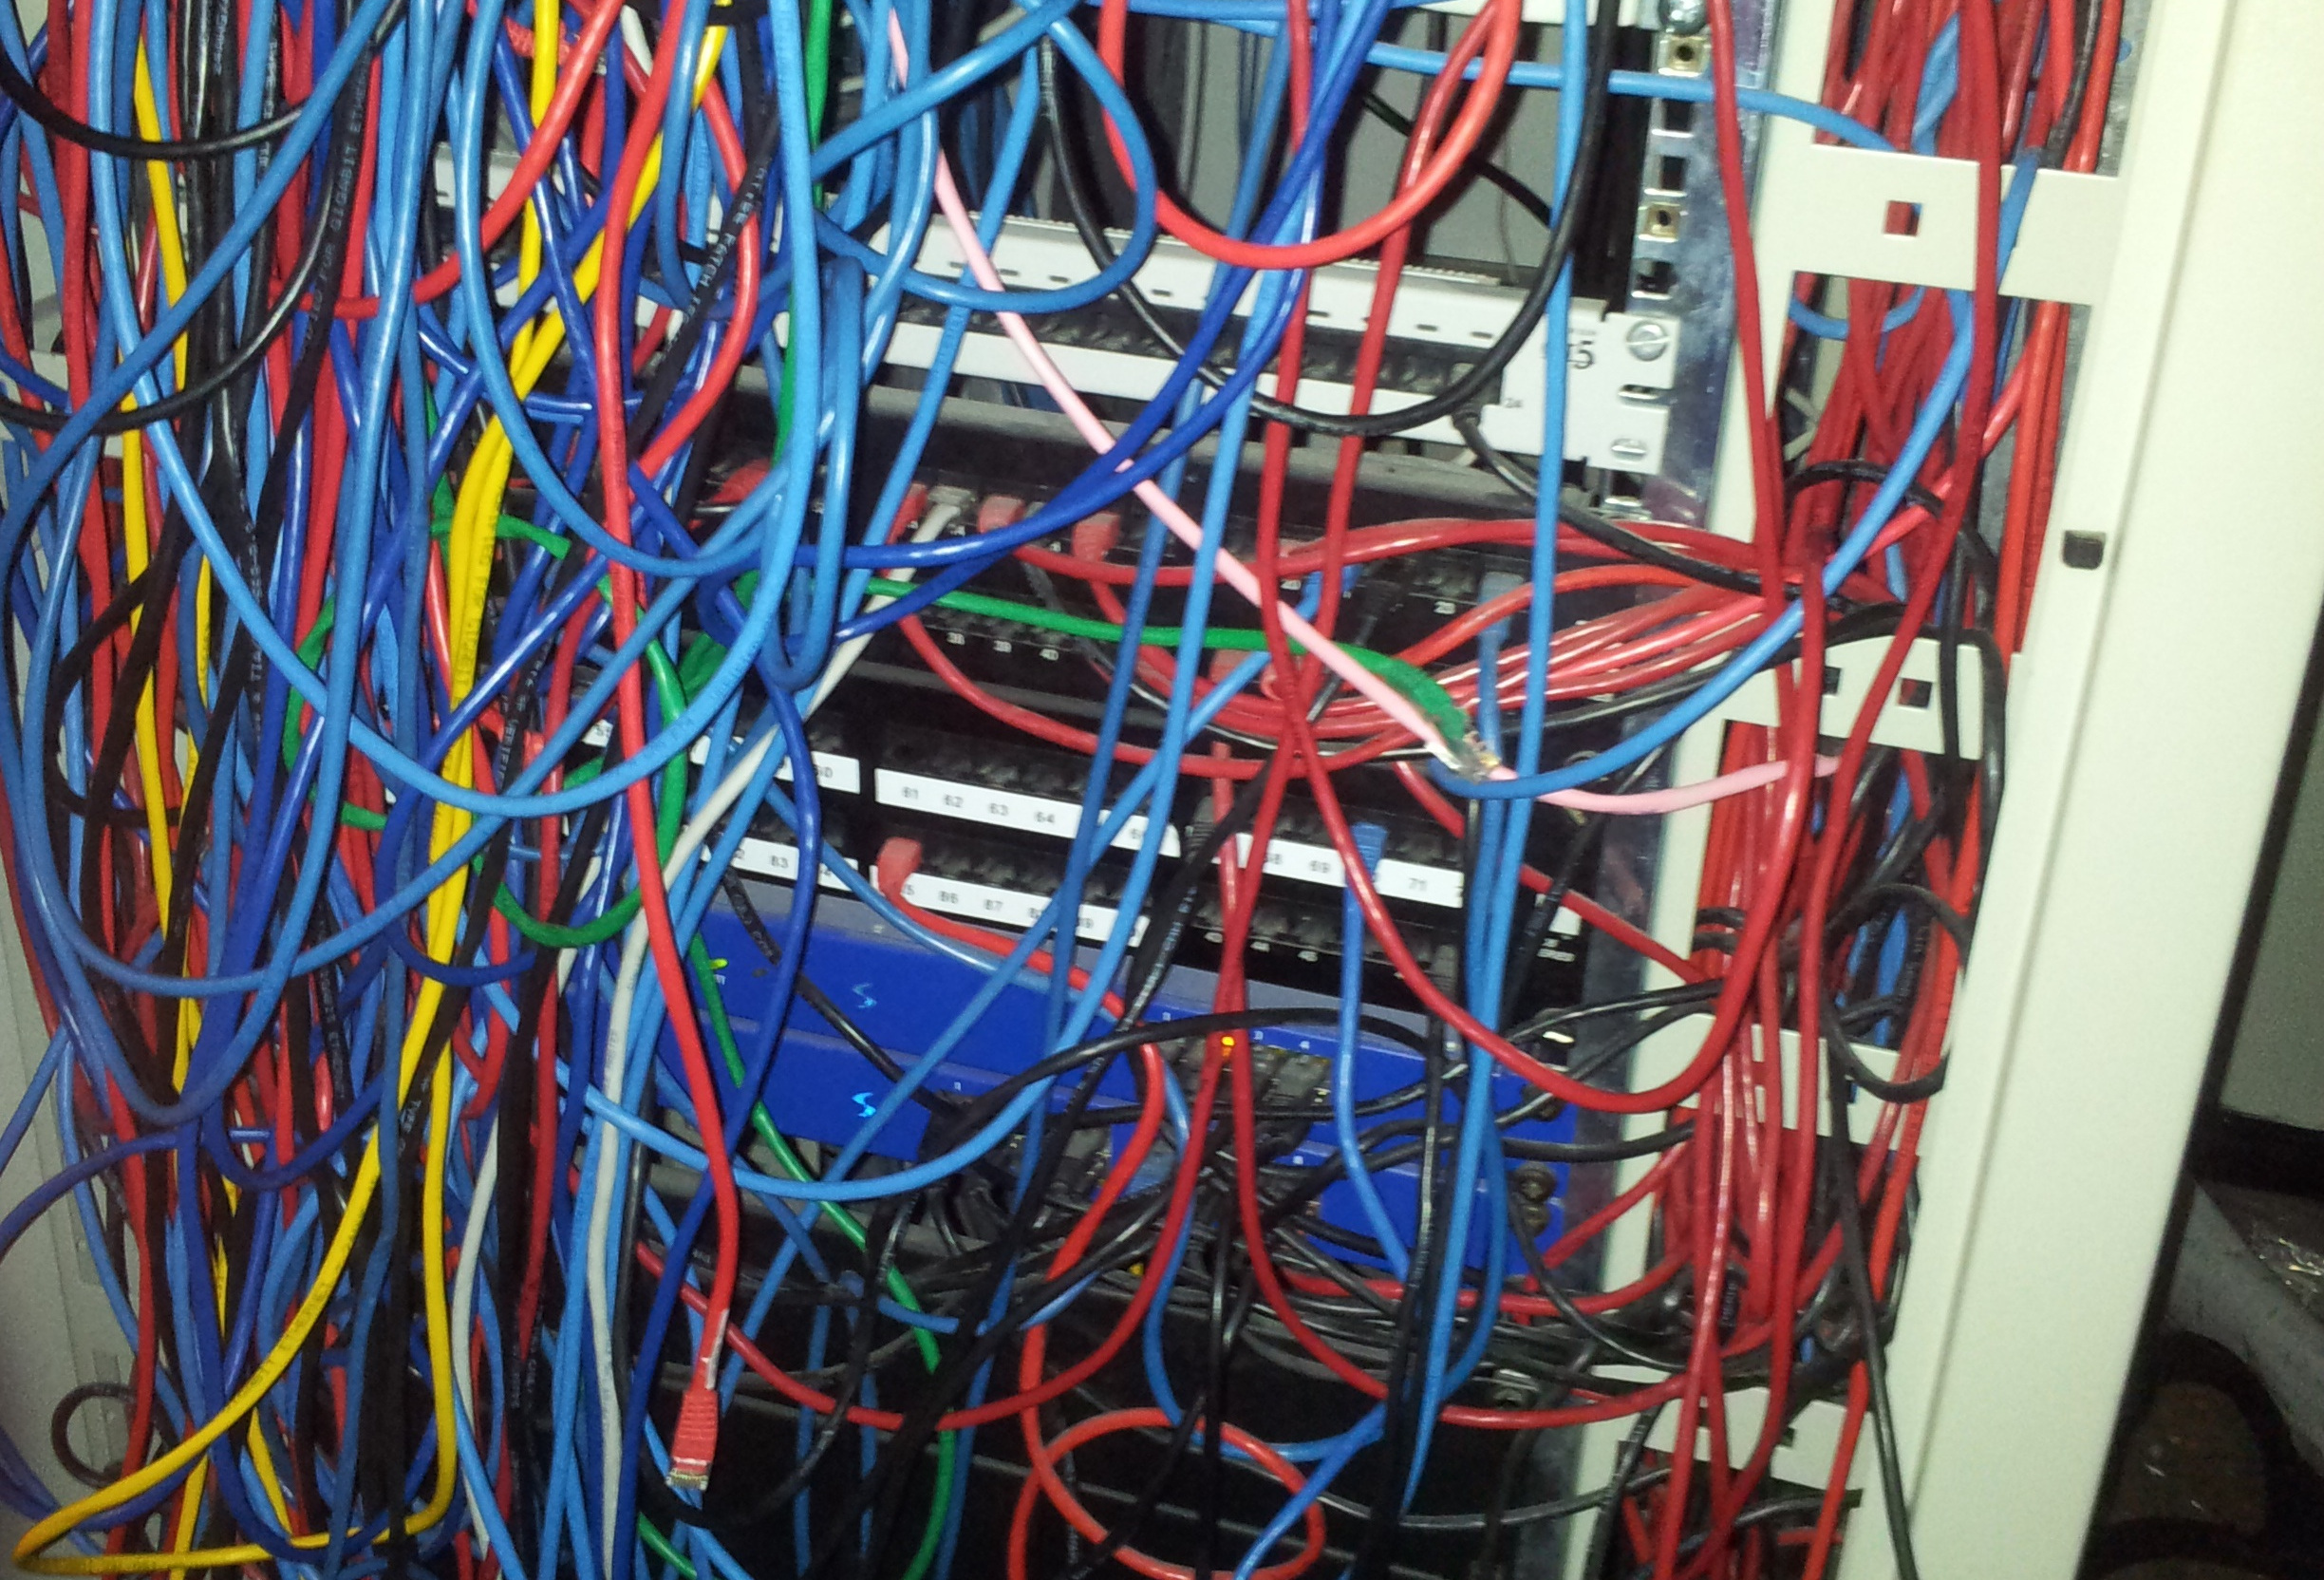
\includegraphics[scale=0.2]{cable-mess.jpg}
    \caption{Pin control in Zephyr < 3.1}
  \end{figure}
\end{frame}

\begin{frame}[fragile]
  \frametitle{Pin Control in Zephyr < 3.1: Example (I)}

  \begin{listing}[H]
    \begin{minted}[fontsize=\tiny]{dts}
      /* boards/arm/nrf52840dk_nrf52840.dts */
      &uart0 {
          ...
          tx-pin = <6>;
          rx-pin = <8>;
          rx-pull-up;
          ...
      };
    \end{minted}
    \begin{minted}[fontsize=\tiny]{c}
      /* drivers/serial/uart_nrfx_uarte.c */
      static int uarte_instance_init(const struct device *dev, ...)
      {
          ...
          nrf_gpio_pin_write(cfg->pseltxd, 1);
          nrf_gpio_cfg_output(cfg->pseltxd);

          if (cfg->pselrxd != NRF_UARTE_PSEL_DISCONNECTED) {
              nrf_gpio_cfg_input(cfg->pselrxd, cfg->rxd_pull);
          }

          nrf_uarte_txrx_pins_set(uarte, cfg->pseltxd, cfg->pselrxd);
          ...
      }
    \end{minted}
    \caption{\textit{Pin control} in nRF, Zephyr 2.7}
  \end{listing}
\end{frame}

\begin{frame}[fragile]
  \frametitle{Pin Control in Zephyr < 3.1: Example (II)}

  \begin{listing}[H]
    \begin{minted}[fontsize=\tiny]{dts}
      /* boards/arm/nucleo_h743zi.dts */
      &usart3 {
          pinctrl-0 = <&usart3_tx_pd8 &usart3_rx_pd9>;
          ...
      };
    \end{minted}
    \begin{minted}[fontsize=\tiny]{c}
      /* drivers/serial/uart_stm32.c */
      static int uart_stm32_init(const struct device *dev)
      {
          ...
          /* Configure dt provided device signals when available */
          err = stm32_dt_pinctrl_configure(config->pinctrl_list, ...);
          ...
      }

      #define STM32_UART_INIT(index)                                       \
          static const struct soc_gpio_pinctrl uart_pins_##index[] =       \
              ST_STM32_DT_INST_PINCTRL(index, 0);                          \
                                                                           \
          static const struct uart_stm32_config uart_stm32_cfg_##index = { \
              ...                                                          \
              .pinctrl_list = uart_pins_##index,                           \
              .pinctrl_list_size = ARRAY_SIZE(uart_pins_##index),          \
          };                                                               \
          ...
    \end{minted}
    \caption{\textit{Pin control} in STM32, Zephyr 2.7}
  \end{listing}
\end{frame}

\begin{frame}[fragile]
  \frametitle{Pin Control in Zephyr < 3.1: Example (III)}

  \begin{listing}[H]
    \begin{minted}[fontsize=\tiny]{c}
      /* boards/arm/mimxrt1010_evk/pinmux.c */
      static int mimxrt1010_evk_init(const struct device *dev)
      {
          ...
          CLOCK_EnableClock(kCLOCK_Iomuxc);
          CLOCK_EnableClock(kCLOCK_IomuxcSnvs);
          ...
          #if DT_NODE_HAS_STATUS(DT_NODELABEL(lpuart1), okay) && CONFIG_SERIAL
            /* LPUART1 TX/RX */
            IOMUXC_SetPinMux(IOMUXC_GPIO_09_LPUART1_RXD, 0);
            IOMUXC_SetPinMux(IOMUXC_GPIO_10_LPUART1_TXD, 0);

            IOMUXC_SetPinConfig(IOMUXC_GPIO_09_LPUART1_RXD,
                                IOMUXC_SW_PAD_CTL_PAD_PKE_MASK |
                                IOMUXC_SW_PAD_CTL_PAD_SPEED(2) |
                                IOMUXC_SW_PAD_CTL_PAD_DSE(6));

            IOMUXC_SetPinConfig(IOMUXC_GPIO_10_LPUART1_TXD,
                                IOMUXC_SW_PAD_CTL_PAD_PKE_MASK |
                                IOMUXC_SW_PAD_CTL_PAD_SPEED(2) |
                                IOMUXC_SW_PAD_CTL_PAD_DSE(6));
          #endif
          ...
      }

      SYS_INIT(mimxrt1010_evk_init, PRE_KERNEL_1, 0);
    \end{minted}
    \caption{\textit{Pin control} in i.MX RT, Zephyr 2.7}
  \end{listing}
\end{frame}

\begin{frame}
  \frametitle{Pin control in Zephyr >= 3.1}

  \begin{itemize}
    \item<1-> Introduced a \textbf{new} \texttt{pinctrl} API in Zephyr 3.0
    \item<2-> \textbf{Standardizes} a few aspects of pin control:
          \begin{itemize}
            \item \textbf{State model}, inspired by Linux Kernel approach
            \item Standardizes \textbf{common properties},
                  e.g.\ \texttt{bias-pull-up}
            \item All \textbf{vendor-specific} bits are contained in
                  \textbf{Devicetree} and a \textbf{SoC specific header}
            \item All \textbf{drivers} use the \textbf{same mechanism} to
                  configure pins
          \end{itemize}
    \item<3-> \texttt{pinctrl} will be \textbf{mandatory} for any new platform
          starting from Zephyr 3.1 onwards
  \end{itemize}

  \begin{figure}
    \centering
    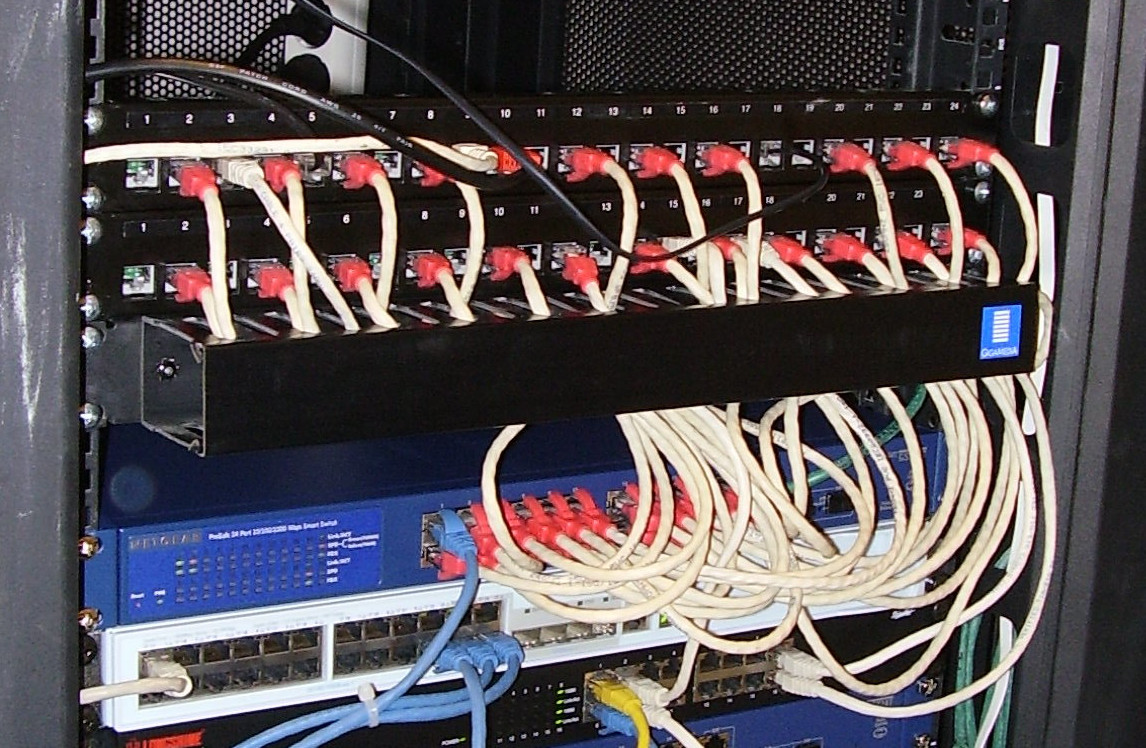
\includegraphics[scale=0.1]{cable-tidy.jpg}
    \caption{Pin control in Zephyr >= 3.1 (CC-BY-SA-4.0, Wikipedia)}
  \end{figure}
\end{frame}

% section: state model ---------------------------------------------------------

\section{State Model}

\begin{frame}
  \begin{center}
    \Huge \textbf{State Model}
  \end{center}
\end{frame}

\begin{frame}
  \frametitle{State Model: Background}

  \begin{itemize}
    \item<1-> Some device drivers need a certain \textbf{pin configuration} to
          be applied to \textbf{work correctly}. This includes
          \textbf{signal multiplexing} and \textbf{other configurations} such as
          pull-up resistors
    \item<2-> Pin configuration \textbf{requirements} may
          \textbf{change at runtime}, e.g.\ when suspending the device
    \item<3-> Each \textbf{required} pin configuration is \textbf{modeled} as a
          state, following Linux Kernel approach
    \item<4-> States \textbf{encode} all necessary pin configurations and are
          \textbf{independent} of each other (they can be applied in any order)
    \item<5-> States \textbf{isolate} driver code from pin configuration:
          \textit{a driver just applies a state}
  \end{itemize}
\end{frame}

\begin{frame}
  \frametitle{State Model: Example}

  \begin{table}
    \centering
    \begin{tabular}{llll}
      \toprule
      \multicolumn{4}{c}{\texttt{I2C0} peripheral (master)}                          \\
      \midrule
      \multicolumn{2}{c}{\texttt{default} state}%
          & \multicolumn{2}{c}{\texttt{sleep} state}                                 \\
      \midrule
      SDA & \tabitem~Pin: PA0                        & SDA & \tabitem~Pin: PA0       \\
          & \tabitem~Drive: Open-Drain               &     & \tabitem~Drive: Default \\
          & \tabitem~Low-Power: No                   &     & \tabitem~Low-Power: Yes \\
      \midrule
      SCL & \tabitem~Pin: PA1                        & SCL & \tabitem~Pin: PA1       \\
          & \tabitem~Drive: Open-Drain               &     & \tabitem~Drive: Default \\
          & \tabitem~Low-Power: No                   &     & \tabitem~Low-Power: Yes \\
      \bottomrule
    \end{tabular}
  \end{table}
\end{frame}

\begin{frame}
  \frametitle{Standard States}

  \begin{itemize}
    \item<1-> In general, pin control states can have \textbf{arbitrary names}
    \item<2-> A \textbf{naming convention} has been established for the most
          \textbf{common} use cases
    \item<3-> Standardization brings \textbf{consistency} and paths for
          \textbf{optimization}. Example: \texttt{sleep} state is automatically
          discarded if \texttt{CONFIG\_PM\_DEVICE=n}
  \end{itemize}

  \begin{adjustwidth}{-0.6cm}{}
    \begin{tabular}{p{0.1\textwidth}p{0.4\textwidth}p{0.5\textwidth}}
      \toprule
      State            & Identifier                       & Purpose                                                                   \\
      \midrule
      \texttt{default} & \texttt{PINCTRL\_STATE\_DEFAULT} & State of the pins when the device is in \textbf{operational} state        \\
      \texttt{sleep}   & \texttt{PINCTRL\_STATE\_SLEEP}   & State of the pins when the device is in \textbf{low power or sleep modes} \\
      \bottomrule
    \end{tabular}
  \end{adjustwidth}
\end{frame}

\begin{frame}
  \frametitle{Custom States}

  \begin{itemize}
    \item<1-> Some device drivers may require \textbf{custom states} beyond
          \texttt{default} or \texttt{sleep}
    \item<2-> \textbf{Solution}: define custom state identifiers named as
          \texttt{PINCTRL\_STATE\_\{NAME\}}, where \texttt{\{NAME\}} is the
          capitalized state name
    \item<3-> It is \textbf{important} that custom state identifiers both are in
          \textbf{driver's scope} and
          \textbf{start from \texttt{PINCTRL\_STATE\_PRIV\_START}} to avoid
          clashes with standard states
  \end{itemize}
\end{frame}

\begin{frame}[fragile]
  \frametitle{Custom States: Example}

  \begin{itemize}
    \item<1-> A device driver needs different states depending on the runtime
          bus operating speed: \textbf{\texttt{slow}} or \textbf{\texttt{fast}}
    \item<2-> \textbf{Solution}: define \texttt{PINCTRL\_STATE\_SLOW} and
          \texttt{PINCTRL\_STATE\_FAST} custom state identifiers
  \end{itemize}

  \begin{listing}[H]
    \begin{minted}[fontsize=\footnotesize]{c}
      /* identifier for 'slow' state */
      #define PINCTRL_STATE_SLOW PINCTRL_STATE_PRIV_START
      /* identifier for 'fast' state */
      #define PINCTRL_STATE_FAST PINCTRL_STATE_PRIV_START + 1
    \end{minted}
    \caption{Identifiers for custom states \texttt{slow} and \texttt{fast}}
  \end{listing}
\end{frame}

\begin{frame}[fragile]
  \frametitle{Skipping states}

  \begin{itemize}
    \item<1-> In some software configurations, certain pin control
          \textbf{states} may be left \textbf{unused}, thus wasting ROM space
    \item<2-> States can be skipped (not stored) if a definition named
          \texttt{PINCTRL\_SKIP\_\{STATE\_NAME\}} \textbf{expanding to 1} is
          in driver's scope when pin control configuration is defined
  \end{itemize}

  \begin{listing}[H]
    \begin{minted}[fontsize=\footnotesize]{c}
      #ifndef CONFIG_PM_DEVICE
      /* If device power management is not enabled, "sleep"
       * state will not be stored, even if defined in Devicetree.
       */
      #define PINCTRL_SKIP_SLEEP 1
      #endif
    \end{minted}
    \caption{\texttt{sleep} state is skipped if \texttt{CONFIG\_PM\_DEVICE=n}}
  \end{listing}
\end{frame}

% section: devicetree representation -------------------------------------------

\section{Devicetree Representation}

\begin{frame}
  \begin{center}
    \Huge \textbf{Devicetree Representation}
  \end{center}
\end{frame}

\begin{frame}[fragile]
  \frametitle{States}

  \begin{itemize}
    \item<1-> Each device's pin control state is represented in Devicetree by
          \textbf{\texttt{pinctrl-N}} properties, where \texttt{N} is the state
          index starting from zero. Property content is vendor specific.
    \item<2-> The \textbf{\texttt{pinctrl-names}} property is then used to
          assign the state to each state property by index
  \end{itemize}

  \begin{listing}[H]
    \begin{minted}[fontsize=\scriptsize]{dts}
      periph0: periph@0 {
          ...
          /* state 0 ("default") */
          pinctrl-0 = <...>;
          ...
          /* state N ("mystate") */
          pinctrl-N = <...>;
          /* names for state 0 up to state N */
          pinctrl-names = "default", ..., "mystate";
          ...
      };
    \end{minted}
    \caption{Pin control states for \texttt{periph0}}
  \end{listing}
\end{frame}

\begin{frame}
  \frametitle{Pin configuration}

  \begin{itemize}
    \item<1-> There are \textbf{multiple} ways to represent the pin
          configurations in Devicetree
    \item<2-> All representations encode the \textbf{same information}: the pin
          multiplexing and the pin configuration parameters
    \item<3-> Representation choice depends largely on
          \textbf{vendor preferences}
    \item<4-> A couple of popular choices: \textbf{grouping} and
          \textbf{node-based}
    \item<5-> \textbf{Standardized properties are mandatory}. For example,
          \texttt{bias-pull-up} has to be used to activate a pin pull-up
          resistor. They are \textbf{pre-defined} in
          \texttt{pincfg-node-group.yaml} or \texttt{pincfg-node.yaml}
  \end{itemize}
\end{frame}

\begin{frame}
  \frametitle{Pin configuration: grouping approach (I)}

  \begin{itemize}
    \item<1-> Multiple signals can be \textbf{grouped} if they share the same
          pin configuration
    \item<2-> Pin configuration parameters for a particular state are enclosed
          in a \textbf{single} Devicetree node
    \item<3-> Platforms using this approach: Atmel, Gigadevice, Nordic,
          NXP\textsuperscript{*}, Raspberry Pi
  \end{itemize}
\end{frame}

\begin{frame}[fragile]
  \frametitle{Pin configuration: grouping approach (II)}

  \begin{listing}[H]
    \begin{minted}[fontsize=\scriptsize]{dts}
      /* board-pinctrl.dtsi */
      #include <vnd-soc-pkgxx.h>
  
      &pinctrl {
          /* Node with pin configuration for default state */
          periph0_default: periph0_default {
              group1 {
                  /* Mappings: PERIPH0_SIGA->PX0, PERIPH0_SIGC->PZ1 */
                  pinmux = <PERIPH0_SIGA_PX0>, <PERIPH0_SIGC_PZ1>;
                  /* Pins PX0 and PZ1 have pull-up enabled */
                  bias-pull-up;
              };
              ...
              groupN {
                  /* Mappings: PERIPH0_SIGB->PY7 */
                  pinmux = <PERIPH0_SIGB_PY7>;
              };
          };
      };
    \end{minted}
    \caption{Pin configuration for \texttt{periph0}, \texttt{default} state}
  \end{listing}
\end{frame}

\begin{frame}[fragile]
  \frametitle{Pin configuration: grouping approach (III)}

  \begin{listing}[H]
    \begin{minted}[fontsize=\scriptsize]{c}
      /* vnd-soc-pkgxx.h */
      ...
      /* encode pinmux entry in a 32-bit field */
      #define VNDSOC_PIN(...)
      ...
      /* valid mappings for SoC package 'xx' (may be autogenerated) */
      #define PERIPH0_SIGA_PX0 VNDSOC_PIN(X, 0, MUX0)
      #define PERIPH0_SIGB_PY7 VNDSOC_PIN(Y, 7, MUX4)
      #define PERIPH0_SIGC_PZ1 VNDSOC_PIN(Z, 1, MUX2)
      ...
    \end{minted}
    \caption{Pre-defined valid mappings for \texttt{periph0} (optional)}
  \end{listing}
\end{frame}

\begin{frame}[fragile]
  \frametitle{Pin configuration: grouping approach (IV)}

  \begin{listing}[H]
    \begin{minted}[fontsize=\scriptsize]{dts}
      /* board.dts */
      #include "board-pinctrl.dtsi"
  
      &periph0 {
          pinctrl-0 = <&periph0_default>;
          pinctrl-names = "default";
      };
    \end{minted}
    \caption{States definition for \texttt{periph0}}
  \end{listing}
\end{frame}

\begin{frame}
  \frametitle{Pin configuration: node approach (I)}

  \begin{itemize}
    \item <1-> A \textbf{state} is assigned with  a \textbf{set of nodes}, each
          one containing the configuration for a single pin
    \item<2-> It requires a \textbf{node per pin and per state} (nodes can not
          be re-used for multiple states)
    \item<3-> \textbf{Recommended} only if nodes can be \textbf{pre-defined},
          it can become too verbose otherwise
    \item<4-> Platforms using this approach: ITE, Microchip, Renesas R-Car,
          SiFive, STM32, TI, ITE
  \end{itemize}
\end{frame}

\begin{frame}[fragile]
  \frametitle{Pin configuration: node approach (II)}

  \begin{listing}[H]
    \begin{minted}[fontsize=\tiny]{dts}
      /* vnd-soc-pkgxx.dtsi
       * File with valid nodes for a specific package (may be autogenerated).
       * This file is optional, but recommended. Note the /omit-if-no-ref/
       * keyword is added to discard node if not used.
       */
 
     &pinctrl {
         /* Mapping for PERIPH0_SIGA -> PX0, to be used for default state */
         /omit-if-no-ref/ periph0_siga_px0_default: periph0_siga_px0_default {
             pinmux = <VNDSOC_PIN(X, 0, MUX0)>;
         };
 
         /* Mapping for PERIPH0_SIGB -> PY7, to be used for default state */
         /omit-if-no-ref/ periph0_sigb_py7_default: periph0_sigb_py7_default {
             pinmux = <VNDSOC_PIN(Y, 7, MUX4)>;
         };
 
         /* Mapping for PERIPH0_SIGC -> PZ1, to be used for default state */
         /omit-if-no-ref/ periph0_sigc_pz1_default: periph0_sigc_pz1_default {
             pinmux = <VNDSOC_PIN(Z, 1, MUX2)>;
         };
     };
    \end{minted}
    \caption{Pre-defined nodes with valid mappings for \texttt{periph0}
      (optional)}
  \end{listing}
\end{frame}

\begin{frame}[fragile]
  \frametitle{Pin configuration: node approach (III)}

  \begin{listing}[H]
    \begin{minted}[fontsize=\scriptsize]{dts}
      /* board-pinctrl.dts */
      #include <vnd-soc-pkgxx.dtsi>

      /* Enable pull-up for PX0 (default state) */
      &periph0_siga_px0_default {
          bias-pull-up;
      };

      /* Enable pull-up for PZ1 (default state) */
      &periph0_sigc_pz1_default {
          bias-pull-up;
      };
    \end{minted}
    \caption{Properties are assigned by board as needed}
  \end{listing}
\end{frame}

\begin{frame}[fragile]
  \frametitle{Pin configuration: node approach (IV)}

  \begin{listing}[H]
    \begin{minted}[fontsize=\scriptsize]{dts}
      /* board.dts */
      #include "board-pinctrl.dtsi"
  
      &periph0 {
          pinctrl-0 = <&periph0_siga_px0_default
                       &periph0_sigb_py7_default
                       &periph0_sigc_pz1_default>;
          pinctrl-names = "default";
      };
    \end{minted}
    \caption{States definition for \texttt{periph0}}
  \end{listing}
\end{frame}

% section: the pin control API -------------------------------------------------

\section{The Pin Control API}

\begin{frame}
  \begin{center}
    \Huge \textbf{The Pin Control API}
  \end{center}
\end{frame}

\begin{frame}
  \frametitle{Pin Control Drivers}

  \begin{itemize}
    \item<1-> There is a single pin control driver per SoC, so it is effectively
          a \textbf{singleton}.
    \item<2-> Pin control drivers only need to implement a \textbf{single}
          function call: \textbf{\texttt{pinctrl\_configure\_pins}}
    \item<3-> \textbf{Vendor specific} bits are defined in
          \textbf{\texttt{pinctrl\_soc.h}}. This header that must be in the
          include path and must define:
          \begin{itemize}
            \item \textbf{\texttt{pinctrl\_soc\_pin\_t}}, the pin configuration
                  opaque type
            \item \textbf{\texttt{Z\_PINCTRL\_STATE\_PINS\_INIT}}, the macro
                  responsible for Devicetree \textit{parsing}
          \end{itemize}
    \item<4-> Reference implementation and test (uses grouping approach):
          \href{https://github.com/zephyrproject-rtos/zephyr/tree/main/tests/drivers/pinctrl/api/src}{\texttt{tests/drivers/pinctrl/api/src}}
  \end{itemize}
\end{frame}

\begin{frame}[fragile]
  \frametitle{Pin Control Drivers: Example (I)}

  \begin{listing}[H]
    \begin{minted}[fontsize=\scriptsize]{yaml}
      ...
      compatible: "vnd,pinctrl"
      ...
      include:
          - name: base.yaml
          - name: pincfg-node-group.yaml
            child-binding:
              child-binding:
                property-allowlist:
                  - bias-pull-down
                  - bias-pull-up

      child-binding:
        child-binding:
          properties:
            pinmux:
              required: true
              type: array
    \end{minted}
    \caption{Example Devicetree binding for a pin control driver (grouping
      approach)}
  \end{listing}
\end{frame}

\begin{frame}[fragile]
  \frametitle{Pin Control Drivers: Example (II)}

  \begin{listing}[H]
    \begin{minted}[fontsize=\scriptsize]{dts}
      /* board-pinctrl.dtsi */
      &pinctrl {
          periph0_default: periph0_default {
              group1 {
                  pinmux = <PERIPH0_SIGA_PA5>,
                           <PERIPH0_SIGB_PA6>;
                  bias-pull-up;
              };
          };
      };

      /* board.dts */
      &periph0 {
          pinctrl-0 = <&periph0_default>;
          pinctrl-names = "default";
      };
    \end{minted}
    \caption{Devicetree definition of \texttt{periph0} default state}
  \end{listing}
\end{frame}

\begin{frame}[fragile]
  \frametitle{Pin Control Drivers: Example (III)}

  \begin{listing}[H]
    \begin{minted}[fontsize=\scriptsize]{c}
      /**
       * State initializer (invoked for every device state)
       *
       * It takes the node stored in prop first index, e.g. for
       * pinctrl-0 'periph0_default', and iterates over its children,
       * i.e. groups. In each group, it iterates over all 'pinmux'
       * elements, using the 'Z_PINCTRL_STATE_PIN_INIT' initializer.
       *
       * @param node_id Device's node (e.g. periph0)
       * @param prop Property holding n-th state, e.g. pinctrl-0
       */
      #define Z_PINCTRL_STATE_PINS_INIT(node_id, prop) \
        {                                              \
            DT_FOREACH_CHILD_VARGS(                    \
              DT_PROP_BY_IDX(node_id, prop, 0),        \
              DT_FOREACH_PROP_ELEM,                    \
              pinmux, Z_PINCTRL_STATE_PIN_INIT         \
            )                                          \
        }
    \end{minted}
    \caption{Example of \texttt{Z\_PINCTRL\_STATE\_PINS\_INIT} macro}
  \end{listing}
\end{frame}

\begin{frame}[fragile]
  \frametitle{Pin Control Drivers: Example (IV)}

  \begin{listing}[H]
    \begin{minted}[fontsize=\scriptsize]{c}
      /** Pin configuration type (here a 32-bit bit field) */
      typedef uint32_t pinctrl_soc_pin_t;

      /**
       * Pin configuration initializer (VND_XXX macros are used to
       * encode configuration in a 32-bit field)
       *
       * @param node_id Group node, e.g. group1
       * @param prop Property holding pinmux (always 'pinmux')
       * @param idx Index of the pinmux element, e.g. 0, 1...
       */
       #define Z_PINCTRL_STATE_PIN_INIT(node_id, prop, idx)    \
          (DT_PROP_BY_IDX(node_id, prop, idx) |                \
           ((VND_PULL_UP * DT_PROP(node_id, bias_pull_up))     \
            << VND_PULL_POS) |                                 \
           ((VND_PULL_DOWN * DT_PROP(node_id, bias_pull_down)) \
            << VND_PULL_POS)                                   \
          ),
    \end{minted}
    \caption{Pin configuration initializer used by
      \texttt{Z\_PINCTRL\_STATE\_PINS\_INIT}}
  \end{listing}
\end{frame}

\begin{frame}[fragile]
  \frametitle{Pin Control Drivers: Example (V)}

  \begin{listing}[H]
    \begin{minted}[fontsize=\scriptsize]{c}
      {
          (PERIPH0_SIGA_PA5 | VND_PULL_UP),
          (PERIPH0_SIGB_PA6 | VND_PULL_UP),
      }
    \end{minted}
    \caption{Result of \texttt{Z\_PINCTRL\_STATE\_PINS\_INIT} when
      invoked for \texttt{periph0}, \texttt{default} state}
  \end{listing}
\end{frame}

\begin{frame}[fragile]
  \frametitle{Using pin control in drivers (I)}

  \begin{itemize}
    \item<1-> Driver binding needs to \textbf{include}
          \texttt{pinctrl-device.yaml}, \textbf{pre-defines}
          \texttt{pinctrl-0..4} and \texttt{pinctrl-names} properties
    \item<2-> \texttt{pinctrl-0} and \texttt{pinctrl-names} properties may
           be flagged as required (improves error diagnostics)
  \end{itemize}

  \begin{listing}[H]
    \begin{minted}[fontsize=\scriptsize]{yaml}
      # vnd,periph.yaml
      ...
      compatible: "vnd,periph"
      ...
      include: [base.yaml, pinctrl-device.yaml]
      ...
    \end{minted}
    \caption{\texttt{vnd,periph} binding includes \texttt{pinctrl-device.yaml}}
  \end{listing}
\end{frame}

\begin{frame}
  \frametitle{Using pin control in drivers (II)}

  \begin{itemize}
    \item<1-> Driver needs to \textbf{define} its pin control configuration by
          using \texttt{PINCTRL\_DT\_DEFINE} or
          \texttt{PINCTRL\_DT\_INST\_DEFINE} macros
    \item<2-> Driver needs to \textbf{keep a reference} to the defined pin
          control configuration by using \texttt{PINCTRL\_DT\_DEV\_CONFIG\_GET}
          or \texttt{PINCTRL\_DT\_INST\_CONFIG\_GET} macros
  \end{itemize}
\end{frame}

\begin{frame}[fragile]
  \frametitle{Using pin control in drivers (III)}
  \begin{listing}[H]
    \begin{minted}[fontsize=\tiny]{c}
      /* A driver for the "vnd,periph" compatible device */
      #define DT_DRV_COMPAT vnd_periph
      ...
      #include <zephyr/drivers/pinctrl.h>
      ...
      struct vnd_periph_config {
          ...
          /* Reference to instance's pinctrl configuration */
          const struct pinctrl_dev_config *pcfg;
      };

      #define VND_PERIPH_DEFINE(i)                                             \
          /* Define pinctrl configuration for instance "i" */                  \
          PINCTRL_DT_INST_DEFINE(i);                                           \
          ...                                                                  \
          static const struct vnd_periph_config vnd_periph_config_##i = {      \
              ...                                                              \
              /* Keep a ref. to the pinctrl configuration for instance "i" */  \
              .pcfg = PINCTRL_DT_INST_DEV_CONFIG_GET(i),                       \
          };                                                                   \
          ...                                                                  \
                                                                               \
          DEVICE_DT_INST_DEFINE(i, vnd_periph_init, NULL, &vnd_periph_data##i, \
                                &vnd_periph_config##i, ...);

      DT_INST_FOREACH_STATUS_OKAY(VND_PERIPH_DEFINE)
    \end{minted}
    \caption{Example of \texttt{vnd,periph} driver defining pin control}
  \end{listing}
\end{frame}

\begin{frame}[fragile]
  \frametitle{Using pin control in drivers (IV)}

  \begin{itemize}
    \item<1-> Driver can apply any defined pin control state by using
        \texttt{pinctrl\_apply\_state}
  \end{itemize}

  \begin{listing}[H]
    \begin{minted}[fontsize=\scriptsize]{c}
      static int vnd_periph_init(const struct device *dev)
      {
          const struct vnd_periph_config *config = dev->config;
          int ret;
          ...
          /* Select "default" state at initialization time */
          ret = pinctrl_apply_state(config->pcfg,
                                    PINCTRL_STATE_DEFAULT);
          if (ret < 0) {
              return ret;
          }
          ...
      }
    \end{minted}
    \caption{\texttt{default} state applied at driver initialization stage}
  \end{listing}
\end{frame}

% section: dynamic pin control -------------------------------------------------

\section{Dynamic Pin Control}

\begin{frame}
  \begin{center}
    \Huge \textbf{Dynamic Pin Control}
  \end{center}
\end{frame}

\begin{frame}
  \frametitle{Dymamic Pin Control}

  \begin{itemize}
    \item<1-> Dynamic pin pontrol refers to the capability of \textbf{changing}
          pin configuration at \textbf{runtime}
    \item<2-> Useful in situations where the \textbf{same firmware} needs to run
          onto \textbf{slightly different} boards
    \item<3-> Can be enabled by setting \texttt{CONFIG\_PINCTRL\_DYNAMIC=y}
    \item<4-> Device pin control configuration is stored in
          \textbf{RAM instead of ROM}, thus allowing state swapping. States are
          still kept in ROM
    \item<5-> An alternative set of states can be set at runtime using
          \texttt{pinctrl\_update\_states}
    \item<6-> Limited to \textbf{uninitialized devices}
  \end{itemize}
\end{frame}

\begin{frame}
  \frametitle{Dymamic Pin Control: Example (I)}

  \begin{itemize}
    \item<1-> \texttt{uart0} is routed to one or another set of pins at boot
          time depending on the Button 1 state.
    \item<2-> \faGithub~\href{https://github.com/zephyrproject-rtos/zephyr/tree/main/samples/boards/nrf/dynamic_pinctrl}{\texttt{samples/boards/nrf/dynamic\_pinctrl}}
  \end{itemize}

  \begin{figure}
    \centering
    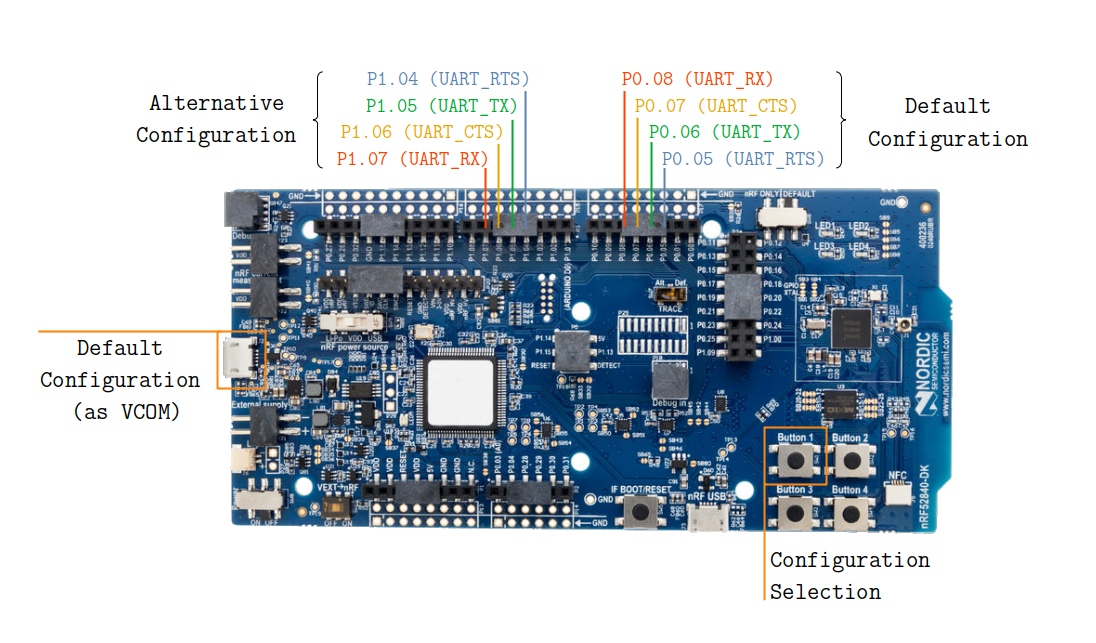
\includegraphics[scale=0.2]{nrf52840dk-dynamic-pinctrl.png}
    \caption{Configuration for nRF52840 DK}
  \end{figure}
\end{frame}

\begin{frame}[fragile]
  \frametitle{Dymamic Pin Control: Example (II)}

  \begin{listing}[H]
    \begin{minted}[fontsize=\scriptsize]{dts}
      / {
          zephyr,user {
              uart0_alt_default = <&uart0_alt_default>;
              uart0_alt_sleep = <&uart0_alt_sleep>;
          };
      };

      &pinctrl {
          /* Alternative pin configuration for UART0 */
          uart0_alt_default: uart0_alt_default {
              group1 {
                  psels = <NRF_PSEL(UART_TX, 1, 5)>,
                          <NRF_PSEL(UART_RTS, 1, 4)>;
              };
              ...
          };
          ...
      };
    \end{minted}
    \caption{Alternative \texttt{uart0} pin configuration defined in Devicetree}
  \end{listing}
\end{frame}

\begin{frame}[fragile]
  \frametitle{Dymamic Pin Control: Example (III)}

  \begin{listing}[H]
    \begin{minted}[fontsize=\scriptsize]{c}
      /* define uart0 alternative configurations (taken from DT) */
      PINCTRL_DT_STATE_PINS_DEFINE(DT_PATH(zephyr_user),
                                   uart0_alt_default);
      #ifdef CONFIG_PM_DEVICE
      PINCTRL_DT_STATE_PINS_DEFINE(DT_PATH(zephyr_user),
                                   uart0_alt_sleep);
      #endif

      /* all uart0 alternative states (default and sleep) */
      static const struct pinctrl_state uart0_alt[] = {
          PINCTRL_DT_STATE_INIT(uart0_alt_default,
                                PINCTRL_STATE_DEFAULT),
      #ifdef CONFIG_PM_DEVICE
          PINCTRL_DT_STATE_INIT(uart0_alt_sleep,
                                PINCTRL_STATE_SLEEP),
      #endif
      };
    \end{minted}
    \caption{Define \texttt{uart0} alternative configurations (taken from DT)}
  \end{listing}
\end{frame}

\begin{frame}[fragile]
  \frametitle{Dymamic Pin Control: Example (IV)}

  \begin{listing}[H]
    \begin{minted}[fontsize=\scriptsize]{c}
      /* declare uart0 device pin control configuration
      * (defined in the driver)
      */
      PINCTRL_DT_DEV_CONFIG_DECLARE(DT_NODELABEL(uart0));

      /* obtain a reference to the uart0 device pin control config */
      struct pinctrl_dev_config *uart0_config =
          PINCTRL_DT_DEV_CONFIG_GET(DT_NODELABEL(uart0));

      /* update uart0 configuration with alternative states */
      pinctrl_update_states(uart0_config, uart0_alt,
                            ARRAY_SIZE(uart0_alt));
    \end{minted}
    \caption{Update \texttt{uart0} states to the alternative set}
  \end{listing}
\end{frame}

\begin{frame}
  \frametitle{Dymamic Pin Control: Example (V)}

  \begin{figure}
    \centering
    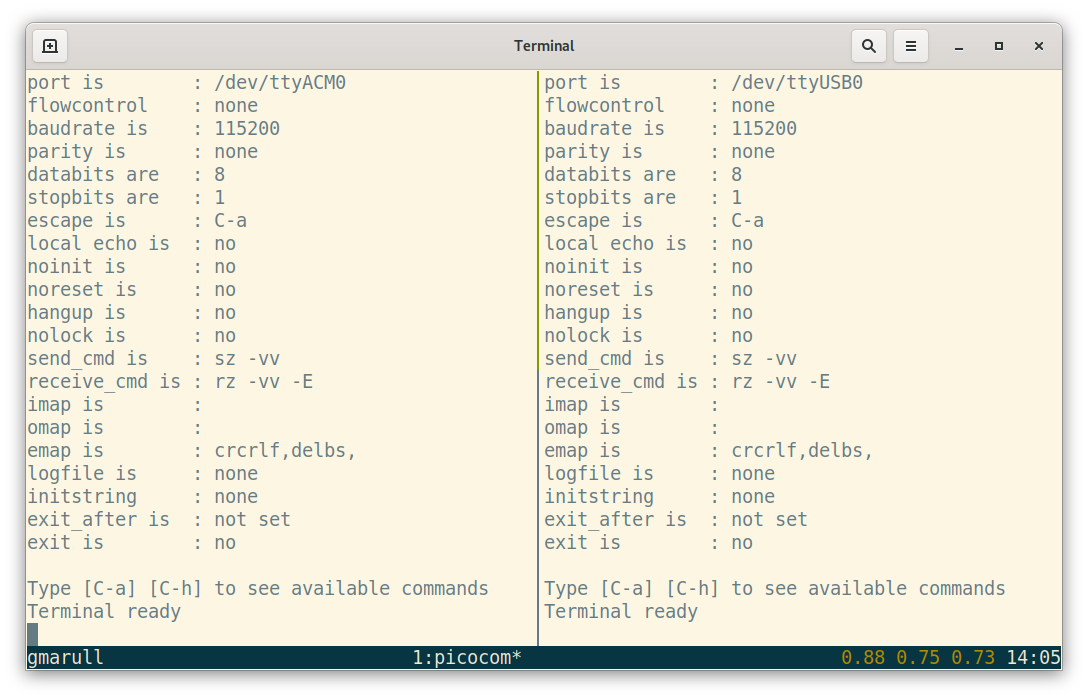
\includegraphics[scale=0.2]{terminals-empty.png}
    \caption{Two serial terminals (left: default, right: alternative)}
  \end{figure}
\end{frame}

\begin{frame}
  \frametitle{Dymamic Pin Control: Example (VI)}

  \begin{figure}
    \centering
    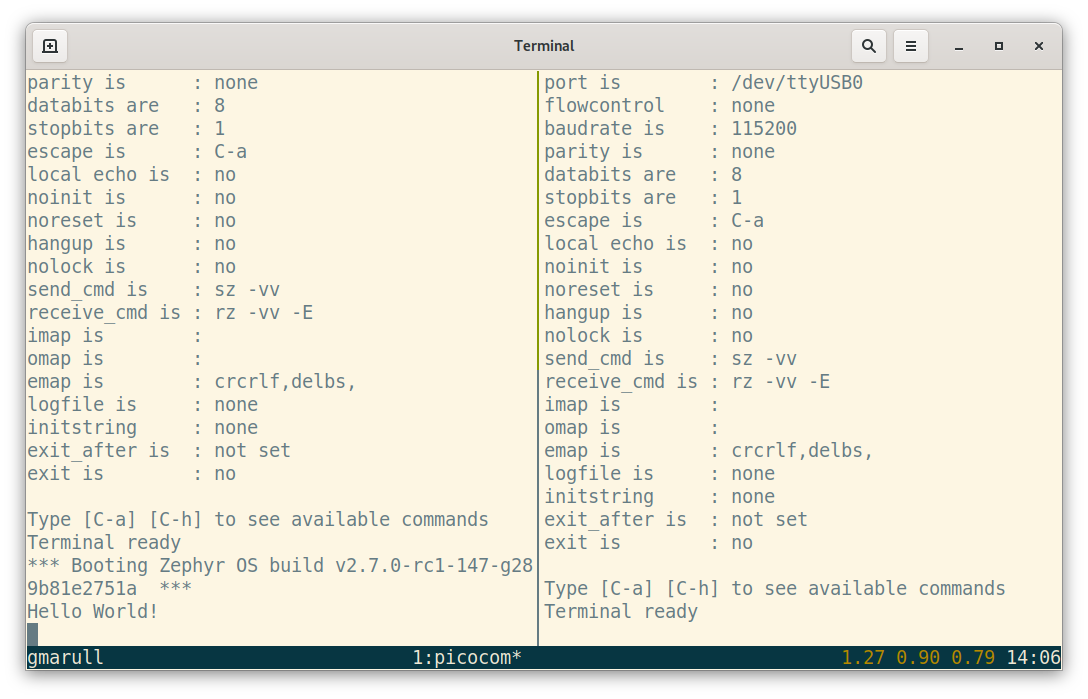
\includegraphics[scale=0.2]{terminals-default.png}
    \caption{Boot without pressing Button 1: \texttt{Hello World!} printed on
      the default set of pins}
  \end{figure}
\end{frame}

\begin{frame}
  \frametitle{Dymamic Pin Control: Example (VII)}

  \begin{figure}
    \centering
    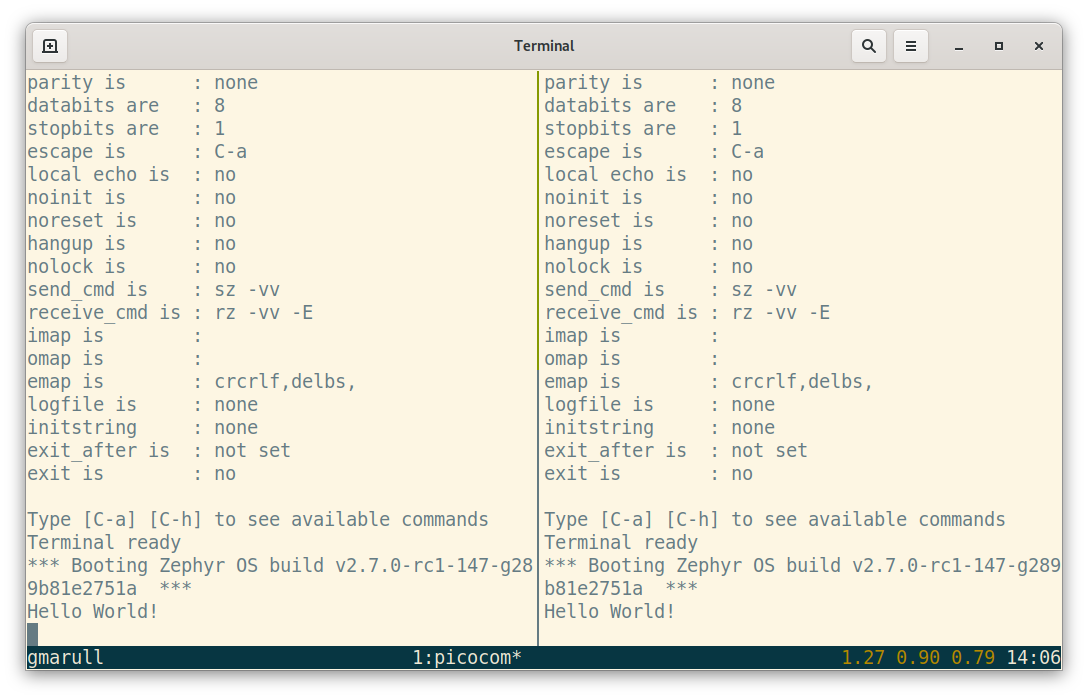
\includegraphics[scale=0.2]{terminals-alt.png}
    \caption{Boot pressing Button 1: \texttt{Hello World!} printed on
      the alternative set of pins}
  \end{figure}
\end{frame}

% section: conclusions ---------------------------------------------------------

\section{Conclusions}

\begin{frame}
  \begin{center}
    \Huge
    \textbf{Conclusions}
  \end{center}
\end{frame}

\begin{frame}
  \frametitle{Conclusions}

  \begin{itemize}
    \item<1-> Pin control is heavily \textbf{vendor dependent}, non-portable
    \item<2-> State model allows to \textbf{isolate} drivers from pin
          configurations, API is used the \textbf{same way} independently of the
          vendor
    \item<3-> State model allows to solve in a \textbf{generic} way problems
          such as pin configuration in \textbf{sleep} or low power modes
    \item<4-> \textbf{Devicetree} representation has been
          \textbf{partially standardized} (common properties,
          e.g.\ \texttt{bias-pull-up})
    \item<5-> All \textbf{vendor specific} bits are contained in
          \textbf{Devicetree} and a \textbf{SoC specific header}
    \item<6-> Even if limited, \textbf{dynamic pin control} allows to route
          peripheral signals to another set of pins at \textbf{runtime}
  \end{itemize}
\end{frame}

\begin{frame}[plain]{}
  \begin{center}
    \huge
    \textbf{THANK YOU!} \\
    Questions? \\
    \vspace{2.5em}
    \normalsize
    \faFilePowerpoint~\url{https://github.com/teslabs/zds-2022-pinctrl} \\
  \end{center}
\end{frame}

\end{document}

